\section{Methods for prediction and analysis of roll damping}
\label{se:methods_for_prediction_and_analysis}
%\subsection{Equations}
%\label{se:equations}
The hydrodynamic governing equation to describe a ship's six degrees of motions when sailing in waters is also written as a damped spring mass equations. In order to limit the scope of the study focusing on the roll damping, the second-order differential equation can be used to model the physical principles of a ship's roll motion response at sea. Then, the roll moment along a longitudinal axis though the centre of gravity can be expressed by,

\input{equations/roll_equation_himeno} 

where $A_{44}$ is the virtual mass moment of inertia, $B_{44}$ is the roll damping moment and $C_{44}$ is the restoring moment. $M_{44}$ represents the external moment (usually moment from external waves), and is of primary interest in this study. For small roll angles, the restoring moments $C_{44}(\phi)$ can be linearized to $C_{1}\phi$. To model the nonlinear restoring moments, $C_{44}(\phi)$ can be described by a n-th order polynomials as $C_{44}(\phi) = C_{1}\phi + C_{2}\phi^2 + C_{3}\phi^3 +, ..., C_{n}\phi^n $

Different experimental test methods are available to obtain the motion signals that can be used to determine the coefficients in Eq.(\ref{eq:roll_equation_himeno}). In this paper, the model scale roll decay tests are used. Since there are no external forces in such tests, the external moment in Eq.(\ref{eq:roll_equation_himeno}) is zero and the governing equation of the tests becomes, 

\begin{equation}
A_{44} \ddot{\phi} + \operatorname{B_{44}}\left(\dot{\phi}\right) + \operatorname{C_{44}}\left(\phi\right) = 0
\end{equation}



where $B_{44}$ can be expressed as expansion series:  
$ B_{44} = B_1\cdot\dot{\phi} + B_2\cdot\dot{\phi}\left|\dot{\phi}\right| + B_3\cdot\dot{\phi}^3 + ... + B_n\cdot\dot{\phi}^n$. Most often, the so-called "linear model", "quadratic model" and "cubic model" are used to represent $B_{44}(\dot{\phi})$ in Eq.(\ref{eq:roll_decay_equation_general_himeno}) by truncating the series to keep only linear, quadratic and cubic terms,

\begin{equation}
A_{44} \ddot{\phi} + B_{1} \dot{\phi} + \operatorname{C_{44}}\left(\phi\right) = 0
\end{equation}

\begin{equation}
A_{44} \ddot{\phi} + \left(B_{1} + B_{2} \left|{\dot{\phi}}\right|\right) \dot{\phi} + \operatorname{C_{44}}\left(\phi\right) = 0
\end{equation}

\input{equations/roll_decay_equation_cubic}


where the $B_1$ and $B_2$ are recognized as the roll damping coefficients.
From roll decay tests, those coefficients are normally derived based on the logarithmic decrements of roll peaks. However, this approach is sensitive to low-frequency disturbances and noises. An alternative and more robust approach, which utilizes full time series of roll decay tests and not only the peaks, is the numerical Parameter Identification Technique (PIT) as described in IMO (2006) and also used in Bulian (2004). In this approach a numerical solution to a one degree of freedom roll equation is fitted to the roll decay time series by tuning the parameters in the roll equation.

\subsection{Estimation of roll damping from roll decay tests}
\label{se:experimental_estimation}
In order to extract roll damping parameters from the roll decay tests, parameters in the cubic, quadratic or linear roll decay models should be identified. The roll angle is measured during the roll decay tests. The system identification is defined as finding the parameters that produce a simulated roll signal that best fits the roll decay test measurement. 
To evaluate the performed tests, a modified version of the PIT approach is developed. This modified approach adds a time-dependent second-degree polynomial to the fitting. It later can be separated from the solution to account for low frequency disturbances. The roll equation that is used for the evaluation has a linear-quadratic damping dependence and a linear restoring term. A quadratic roll damping model can be linearized using the equivalent linear damping coefficient \parencite{himeno_prediction_1981}:

\begin{equation}
B_{e} = B_{1} + \frac{8 B_{2} \omega_{0} \phi_{a}}{3 \pi}
\end{equation}


In order to obtain the damping coefficients $B_1$ and $B_2$, roll damping is calculated for two or more roll amplitudes $\phi_a$ for the same motion frequency (for this study, it is referred to the natural frequency $\omeg$ because free roll decay tests were used for the model tests.). $B_1$ and $B_2$ is obtained by fitting equation \ref{eq:B_e_equation} to this data as shown in figure \ref{fig:ikeda_B_1_B2}.  

\begin{figure}[H]
    \centering
    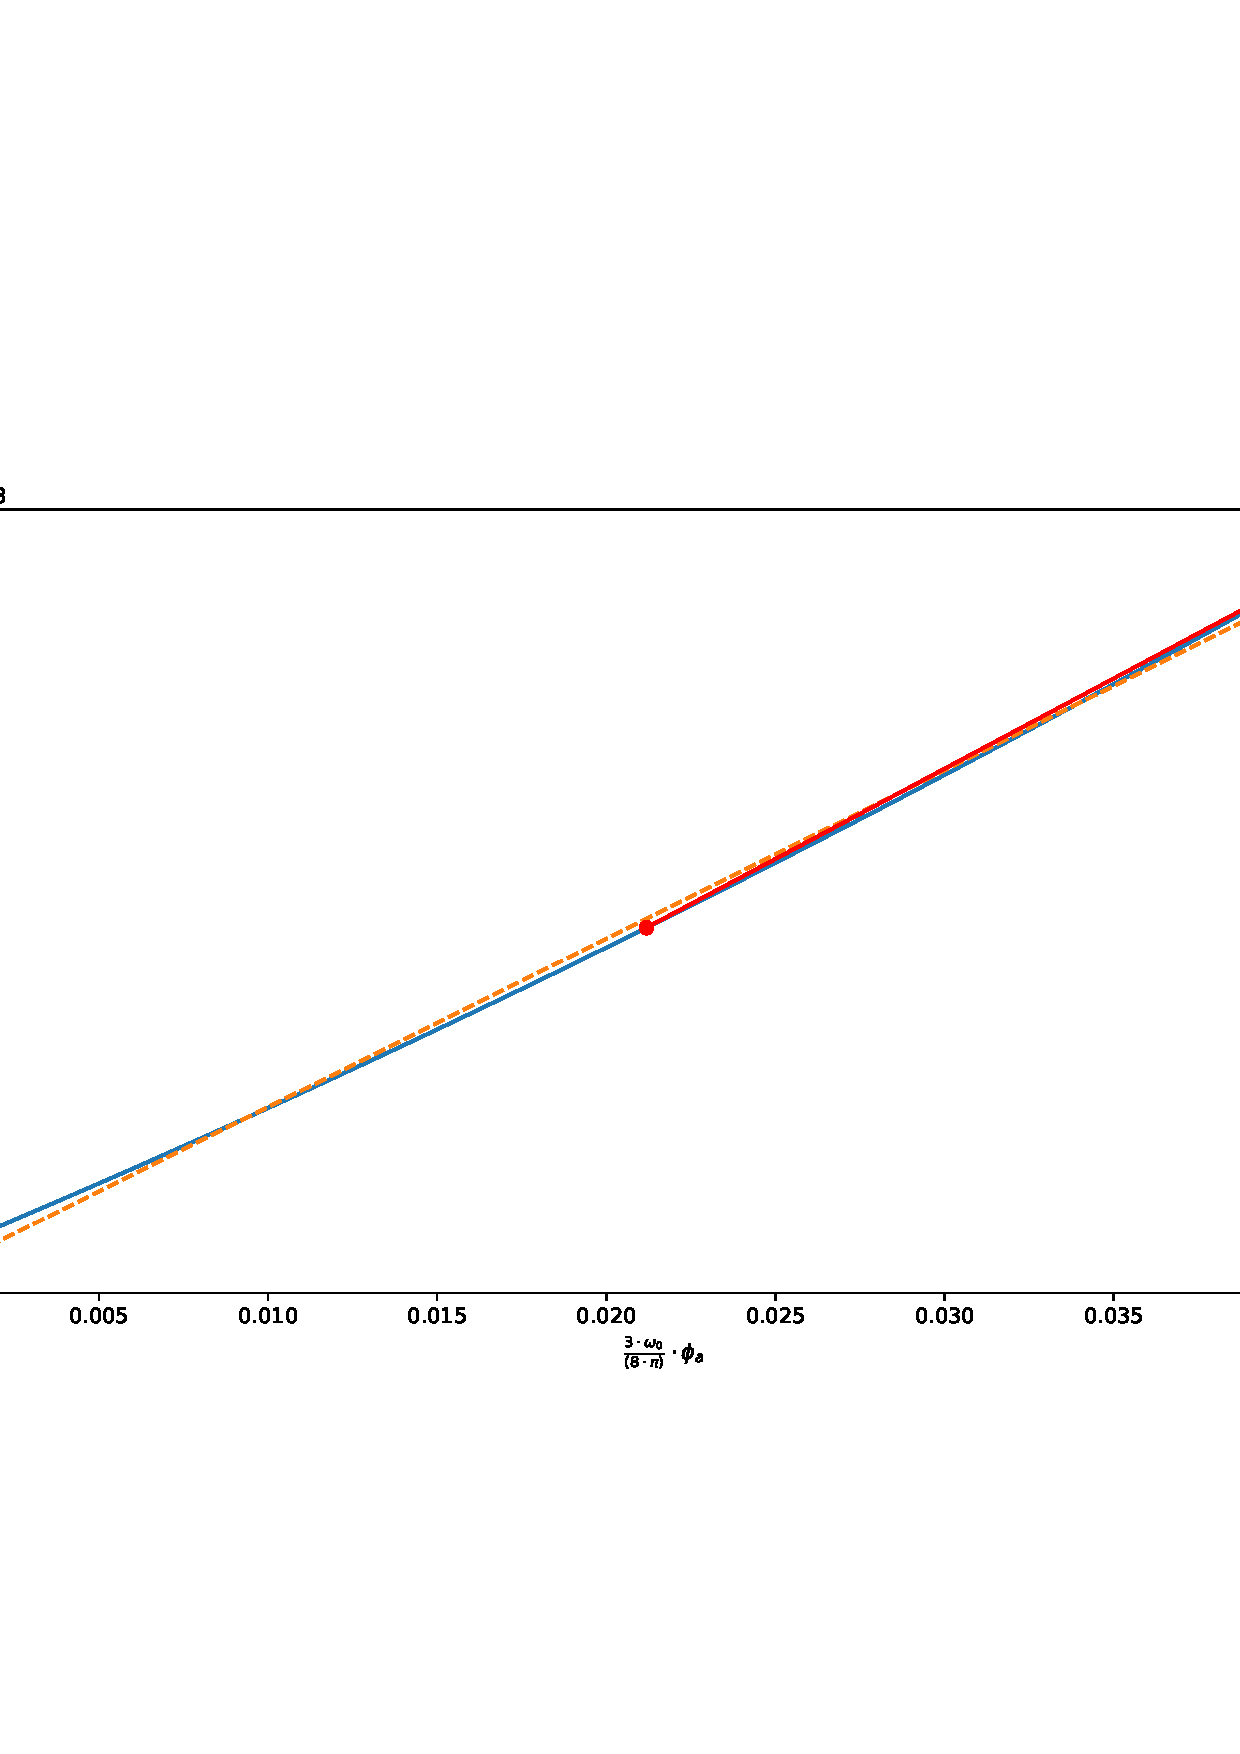
\includegraphics[height=5cm, width=8cm]{figures/ikeda_B_1_B_2.pdf}
    \vspace{-0.5cm}
    \caption{Variation of roll amplitude to derive $B_1$ and $B_2$}
    \label{fig:ikeda_B_1_B2}
\end{figure}




%Peter Piehl \parencite{henry_peter_piehl_ship_nodate} shows an analytical solution %to the linear model in equation \ref{eq:roll_decay_equation_himeno_linear}, %where the natural frequency of the motion is obtained by:
%\begin{equation}
\omega_{0} = \sqrt{\frac{C}{A_{44}}}
\end{equation}

%
%The roll damping and the natural frequency can be made non dimensional using %the following expressions \parencite{himeno_prediction_1981}: 
%\input{equations/B44_hat_equation}
%\begin{equation}
\omega_{hat} = \frac{\sqrt{2} \omega \sqrt{\frac{beam}{g}}}{2}
\end{equation}

%The ordinary differential equations for roll motion in equation \ref{eq:roll_decay_equation_cubic}, \ref{eq:roll_decay_equation_himeno_quadratic} and \ref{eq:roll_decay_equation_himeno_linear} are solved numerically using Explicit Runge-Kutta method of order 5(4). 

%Figure \ref{fig:analytical} shows a comparison for the linear model between this kind of numerical solution and the exact analytical solution \parencite{henry_peter_piehl_ship_nodate}. It seems that the numerical solution agrees well with the analytical. 

%\begin{figure}[h]
%    \centering
%    \includegraphics[width=\columnwidth]{figures/analytical.pdf}
%    \caption{Analytical and numerical solution to the linear model}
%    \label{fig:analytical}
%\end{figure}


%\subsection{Parameter Identification Technique}
%\label{se:PIT}
It should be noted that even though the approach could well handle roll equations with higher order of non-linearities in the damping term as well as a non-linear restoring term, the limited amplitudes at which the roll decay tests were conducted cannot motivate advantages of higher order models. 
The goodness of the fit is described using the coefficient of determination:
\begin{equation} \label{eq:R2}
R^2=1-\frac{SS_{res}}{SS_{tot}}
\end{equation}
where $SS_{res}$ is sum of squares of residuals and $SS_{tot}$ is total sum of squares. Two different solution approaches have been investigated for the system identification: a "Derivation approach" and an "Integration approach". 
The "Derivation approach" has the advantage of being very much faster than the "Integration approach" but also the disadvantage of needing to calculate the numerical derivatives which for measurement data also requires some low pass filtration. The "Integration approach" may however also have a disadvantage of not converging.



In the "Derivation approach" the first and second roll time derivatives are calculated numerically so that the parameters in the models are the only unknowns and the optimal parameters that gives the best fit can simply be determined using a least square fit.
In the "Integration approach" the parameters are found by solving a nonlinear least-squares problem using the least-square method \parencite{noauthor_scipyoptimizeleast_squares_nodate} and the Trust Region Reflective algorithm with smooth approximation of l1 (absolute value). This approach requires that ordinary differential equation is solved for many "guessed" sets of parameters till the solution converges.

\begin{figure}[H]
    \centering
    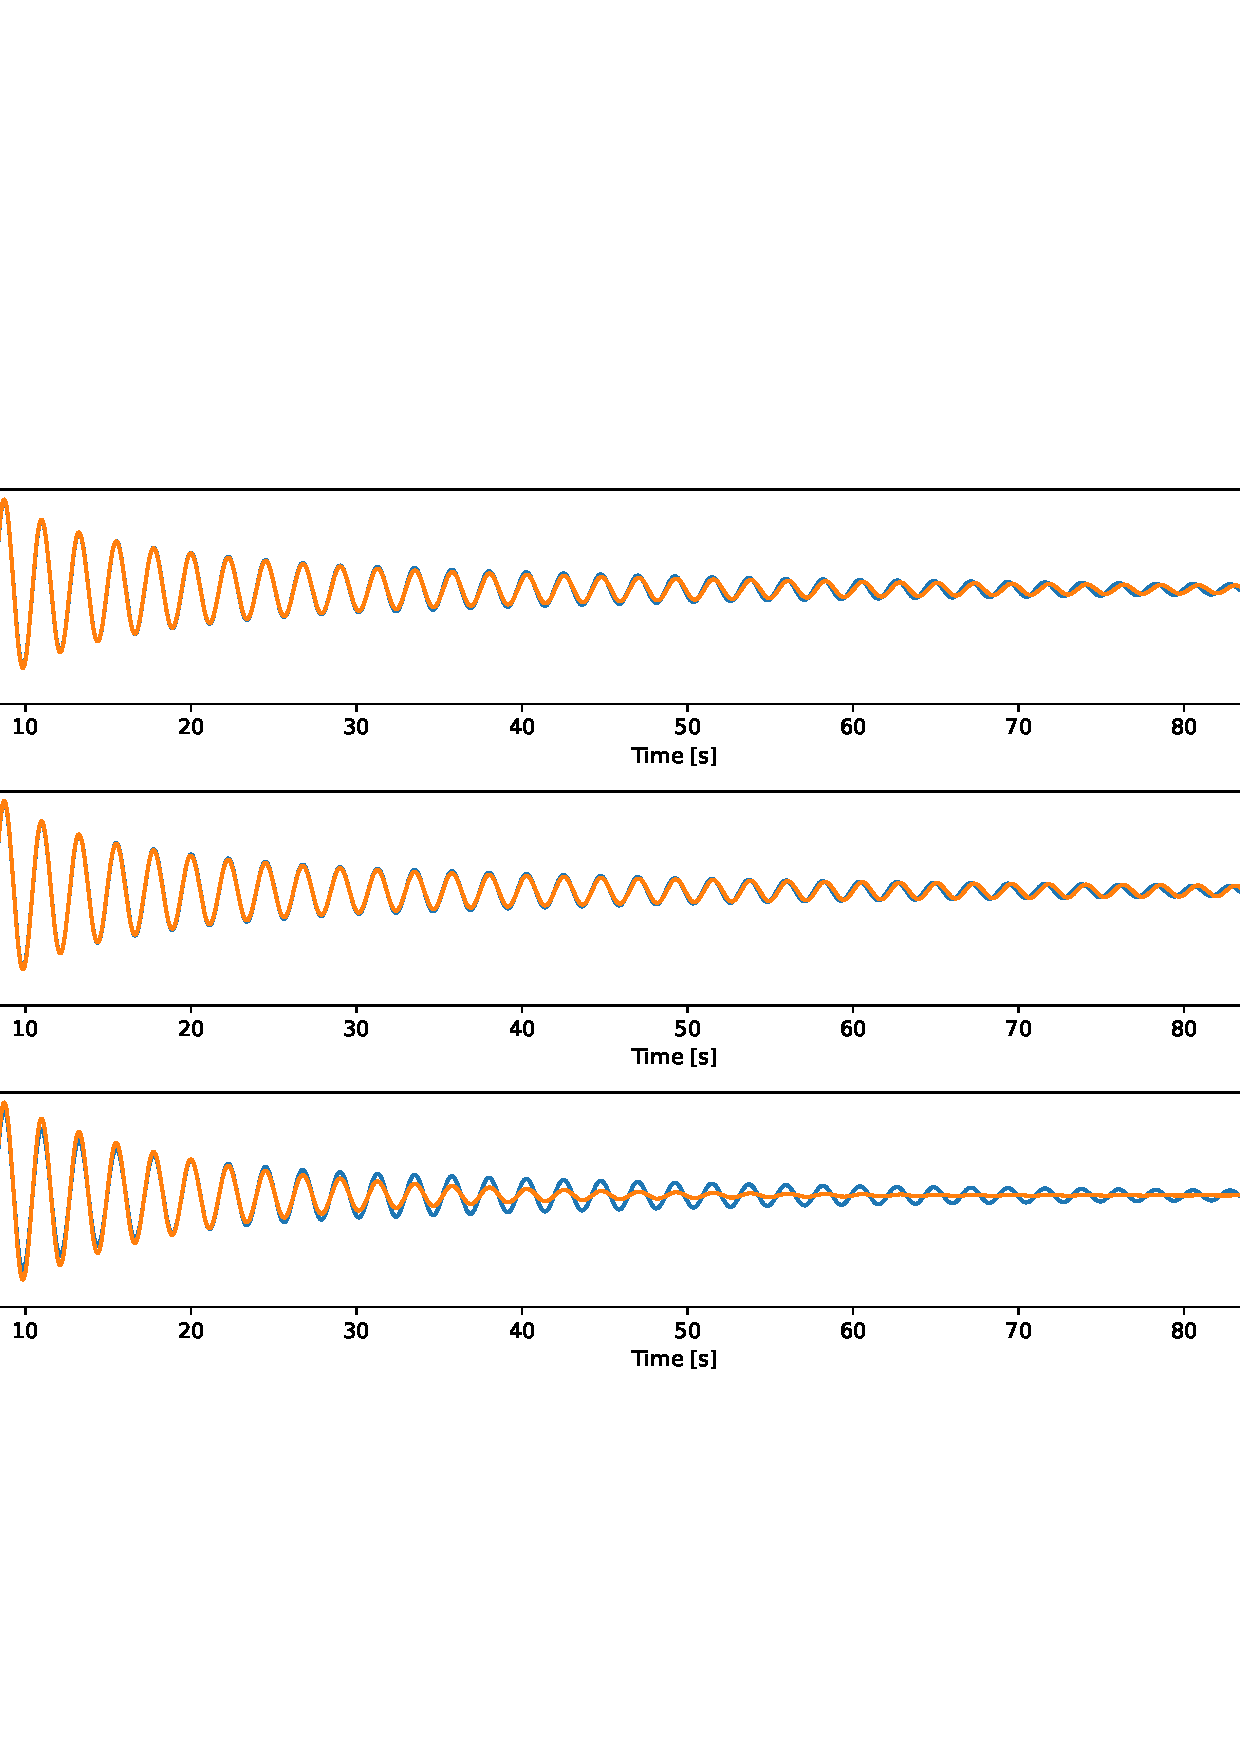
\includegraphics[width=12cm, height = 6cm ]{figures/roll_decay_model_compare.pdf}
    \caption{Roll decay test comparison of linear, quadratic and cubic model}
    \label{fig:roll_decay_model_compare}
\end{figure}

A validation of the developed system identification method has been conducted by checking that known parameters from signals from simulations with the linear, quadratic and cubic models can all be identified. For example,
Figure \ref{fig:roll_decay_model_compare} shows a comparison between the linear, quadratic and cubic model for a random chosen roll decay test motion results. It can be seen that the linear model can not give a perfect representation for the whole range of roll angles.    




\subsection{Ikeda's method: from strip theory to semi-empirical formulas}
\label{se:semi-empirical methods}
Since the scale effect of the damping is mainly associated with the skin friction on ship hulls and the friction only contributes very little to a ship's total roll damping, the most reliable way to obtain a ship's roll damping coefficients is to carry out model scale experimental tests. 
While in a ship's early design stage when only limited information is available and flexible to be adjusted, such as the ship's principal dimensions and the basic hull geometry, some semi-empirical methods were also proposed to predict the roll damping (\cite{himeno_prediction_1981}). The most recognize method was developed in a series of research articles (\cite{ikeda_roll_1978}, \cite{ikeda_eddy_1978}, \cite{ikeda_roll_1979}, \cite{ikeda_components_1978}, \cite{ikeda_velocity_1979}), and it is well-known to be named as Ikeda's method. This method divides the roll damping into five damping components, i.e., the friction component $B_F$, the eddy component $B_e$, the lift component $B_L$, the wave component $B_W$ and the bilge keel component $B_BK$, as in the following Eq.(\ref{eq:ikeda}), 

\begin{equation} \label{eq:ikeda}
B = B_F + B_E + B_L + B_W + B_{BK}
\end{equation}

where the wave and eddy components require strip method calculations to get the ship's shape coefficients. This is not an attractive option for the present study since that would require calculations with exact hull geometries to be carried out for all of the ships in the study. There exist however a \emph{Simplified Ikeda method} \cite{kawahara_simple_2011} that is instead used in this study to calculate the eddy component $B_E$ and wave component $B_W$. Figure \ref{fig:ikeda_vs_simplified} shows a comparison between roll damping components calculated with \emph{Ikeda} and \emph{Simplified Ikeda method}. The roll damping is under-predicted with the simplified method for this particular case which is expected according to the limitations of this method  \cite{kawahara_simple_2011}.



The roll damping consists of linear and nonlinear components. At zero speed the nonlinear damping is caused by the two-dimensional separation at the bilge keel or near the bilge circle (Eddy damping $B_E$). While at speed the nonlinear damping is mainly caused by the hydrodynamic lift force on the hull, represented as lift damping $B_L$. $B_E$ vanishes at high speed ($F_n>0.15)$ \cite{ikeda_components_1978}.

The wave damping also changes at speed. Ikeda \cite{ikeda_components_1978} proposes a formula for the fraction between wave damping at speed and zero speed: $\frac{B_W}{B_{W0}}$

The Ikeda method has been used to calculate the roll damping for a PCTC vessel Faust \cite{soder_assessment_2019}.


%\begin{figure}[h]
%    \centering
%    \includegraphics[width=\columnwidth]{figures/ikeda_faust.pdf}
%    \caption{Roll damping components calculated with Ikeda method for PCTC Faust}
%    \label{fig:ikeda_faust}
%\end{figure}





\begin{figure}[h]
    \centering
    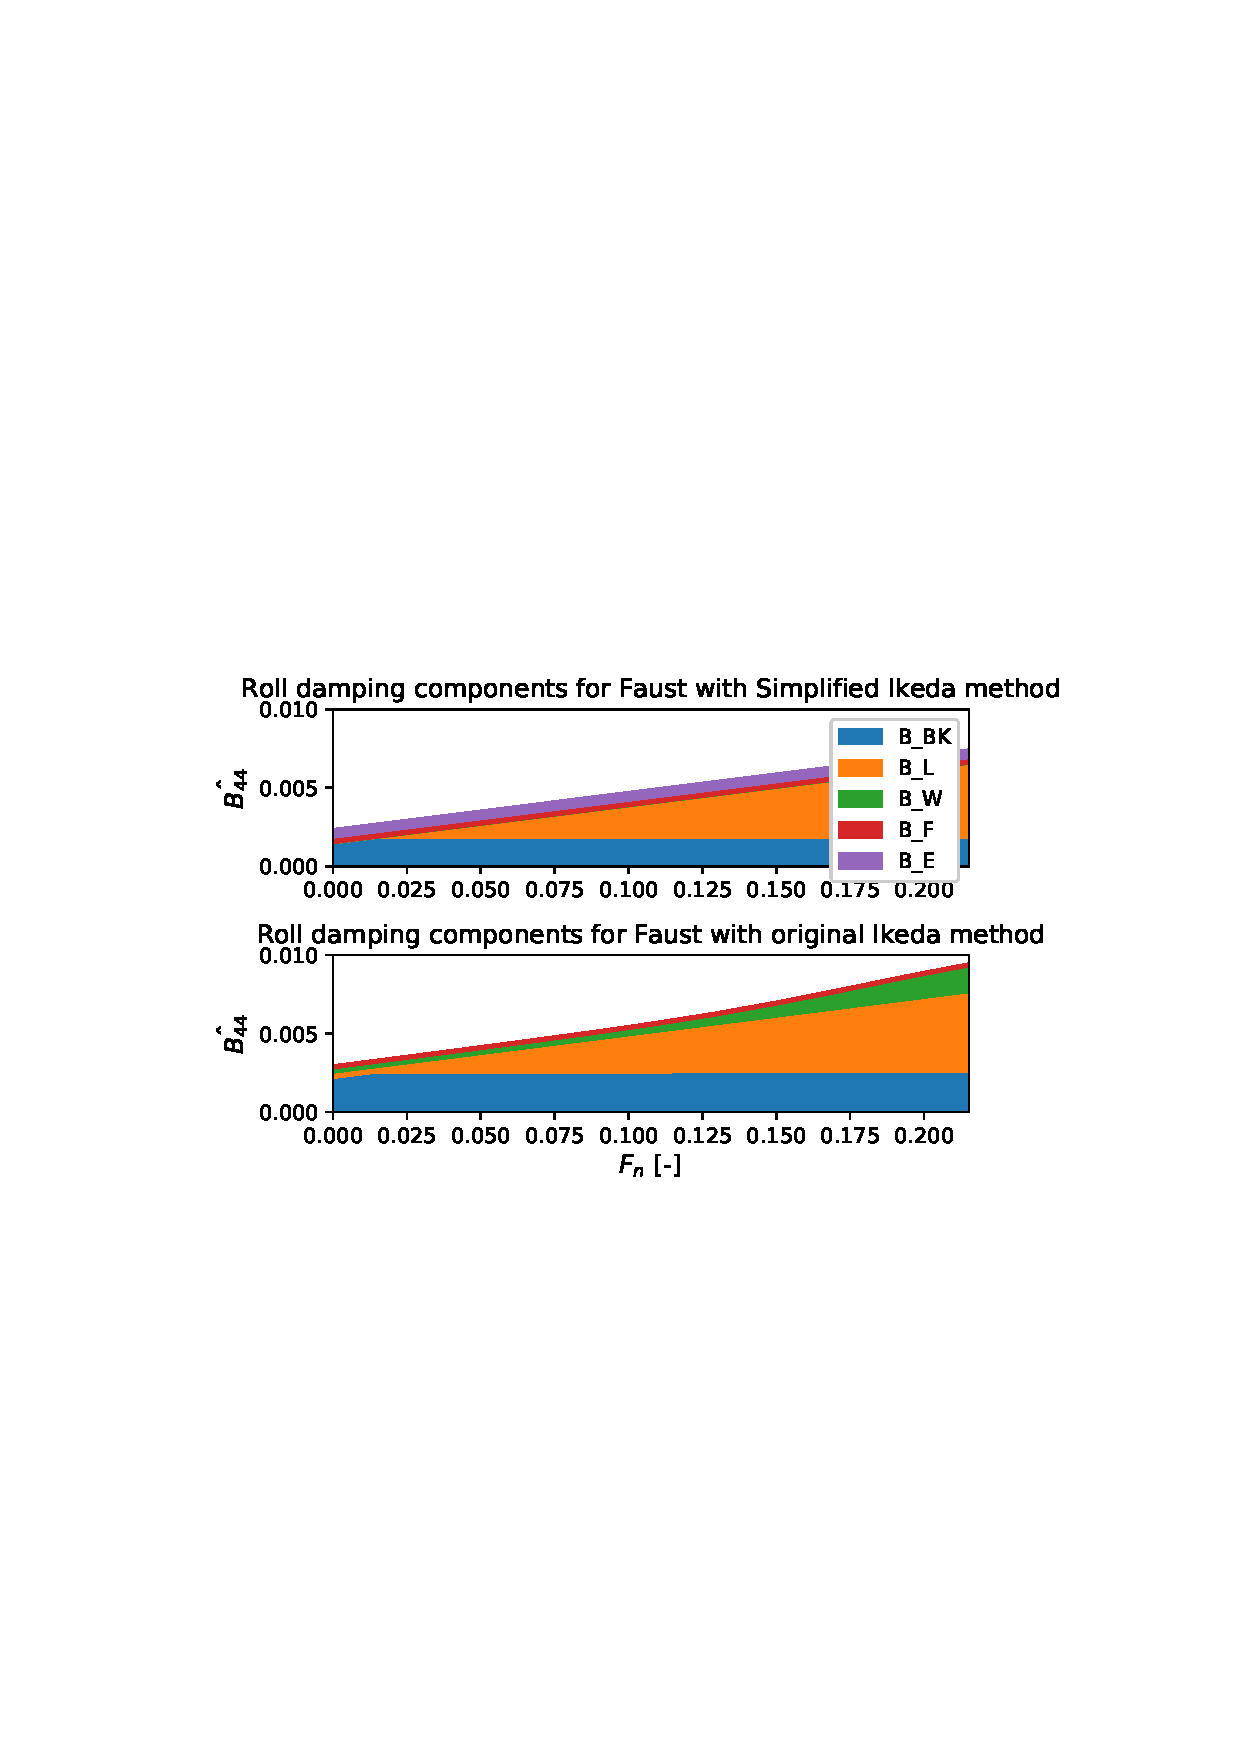
\includegraphics[height=7cm, width=14cm]{figures/ikeda_vs_simplified.pdf}
    \caption{Roll damping components calculated with Ikeda and Simplified Ikeda for PCTC Faust}
    \label{fig:ikeda_vs_simplified}
\end{figure}

The Simplified Ikeda method \cite{kawahara_simple_2011} has been implemented \cite{alexandersson_martinlarsalbertrolldecay-estimators_2020} with the intention to be used both as a benchmark and maybe also as a sub-component of a new method. The examples from \cite{kawahara_simple_2011} was recalculated to check that the method has been implemented correctly. The authors have been unable to find other ways to validate the implementation, which introduces some uncertainty to the comparisons. The method has been implemented as a function where the total roll damping and its component is calcultated: 
\begin{equation} \label{eq:simplified_ikeda_equation}
\left[\  B_{F}, \  B_{W}, \  B_{E}, \  B_{BK}, \  B_{L}\right] = f\left(L_{pp},B,T,C_{b},A_{0},OG,\phi_{a},BK_{L},BK_{B},\omega,V\right)
\end{equation}


A quadratic roll damping model can be linearized using the equivalent linear damping coefficient \cite{himeno_prediction_1981}:
\begin{equation}
B_{e} = B_{1} + \frac{8 B_{2} \omega_{0} \phi_{a}}{3 \pi}
\end{equation}

In order to obtain the damping coefficients $B_1$ and $B_2$ in the quadratic model in equation \ref{eq:roll_decay_equation_himeno_quadratic} roll damping is calculated for two or more roll amplitudes ($\phi_a$). $B_1$ and $B_2$ is obtained by fitting equation \ref{eq:B_e_equation} to this data as shown in figure \ref{fig:ikeda_B_1_B2}.  

A parameter variation was conducted in order to study the simplified method.
A "median ship" with the most usual parameters in the database was chosen as the baseline of the variation. The parameters were varied to the extreme values of the database, see figure \ref{fig:ship_parameters} for more details. 

Figure \ref{fig:ikeda_variation} shows this variation where all parameters have been none dimensionalized using froude scaling with $L_{pp}$ as scale factor. 
It seems that length to beam ratio between 0.23 and 0.24 has a huge peak. Also length to draft ratio below 0.034 has a large peak. 

\begin{figure}[H]
    \centering
    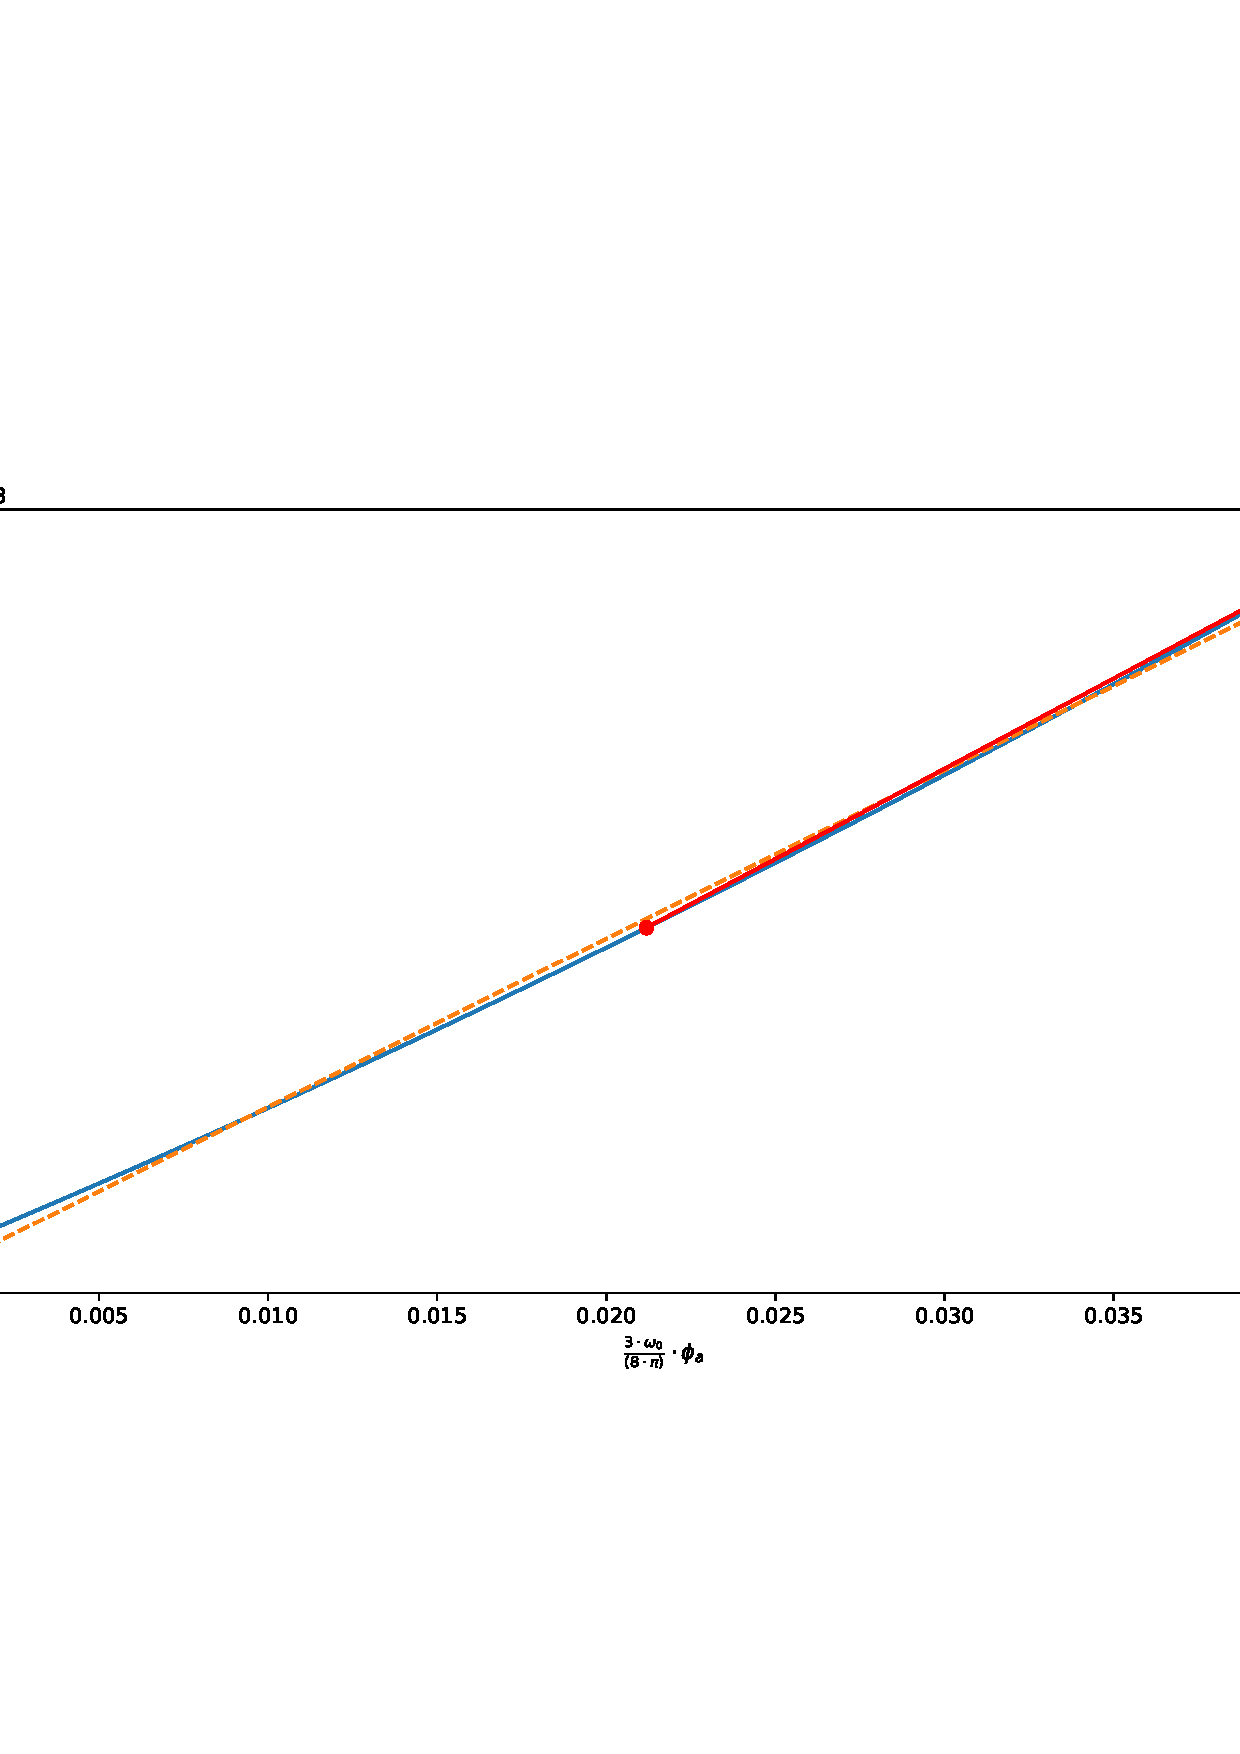
\includegraphics[height=5cm, width=8cm]{figures/ikeda_B_1_B_2.pdf}
    \vspace{-0.5cm}
    \caption{Variation of roll amplitude to derive $B_1$ and $B_2$}
    \label{fig:ikeda_B_1_B2}
\end{figure}

\begin{figure}[H]
    \centering
    \includegraphics[height=13cm, width=15cm]{figures/ikeda_variation.pdf}
    \caption{Simplified method parameter variation}
    \label{fig:ikeda_variation}
\end{figure}


\subsection{Simplified Ikeda's method: semi-empirical formulas}
\label{se:simplified_ikeda}
The Simplified Ikeda method \parencite{kawahara_simple_2011} has been implemented \parencite{alexandersson_martinlarsalbertrolldecay-estimators_2020} with the intention to be used both as a benchmark and maybe also as a sub-component of a new method. The examples from \parencite{kawahara_simple_2011} was recalculated to check that the method has been implemented correctly. The authors have been unable to find other ways to validate the implementation, which introduces some uncertainty to the comparisons. The method has been implemented as a function where the total roll damping and its component is calcultated: 
\begin{equation} \label{eq:simplified_ikeda_equation}
\left[\  B_{F}, \  B_{W}, \  B_{E}, \  B_{BK}, \  B_{L}\right] = f\left(L_{pp},B,T,C_{b},A_{0},OG,\phi_{a},BK_{L},BK_{B},\omega,V\right)
\end{equation}


A quadratic roll damping model can be linearized using the equivalent linear damping coefficient \parencite{himeno_prediction_1981}:
\begin{equation}
B_{e} = B_{1} + \frac{8 B_{2} \omega_{0} \phi_{a}}{3 \pi}
\end{equation}

In order to obtain the damping coefficients $B_1$ and $B_2$ in the quadratic model in equation \ref{eq:roll_decay_equation_himeno_quadratic} roll damping is calculated for two or more roll amplitudes ($\phi_a$). $B_1$ and $B_2$ is obtained by fitting equation \ref{eq:B_e_equation} to this data as shown in figure \ref{fig:ikeda_B_1_B2}.  

A parameter variation was conducted in order to study the simplified method.
A "median ship" with the most usual parameters in the database was chosen as the baseline of the variation. The parameters were varied to the extreme values of the database, see figure \ref{fig:ship_parameters} for more details. 

Figure \ref{fig:ikeda_variation} shows this variation where all parameters have been none dimensionalized using froude scaling with $L_{pp}$ as scale factor. 
It seems that length to beam ratio between 0.23 and 0.24 has a huge peak. Also length to draft ratio below 0.034 has a large peak. 

\begin{figure}[H]
    \centering
    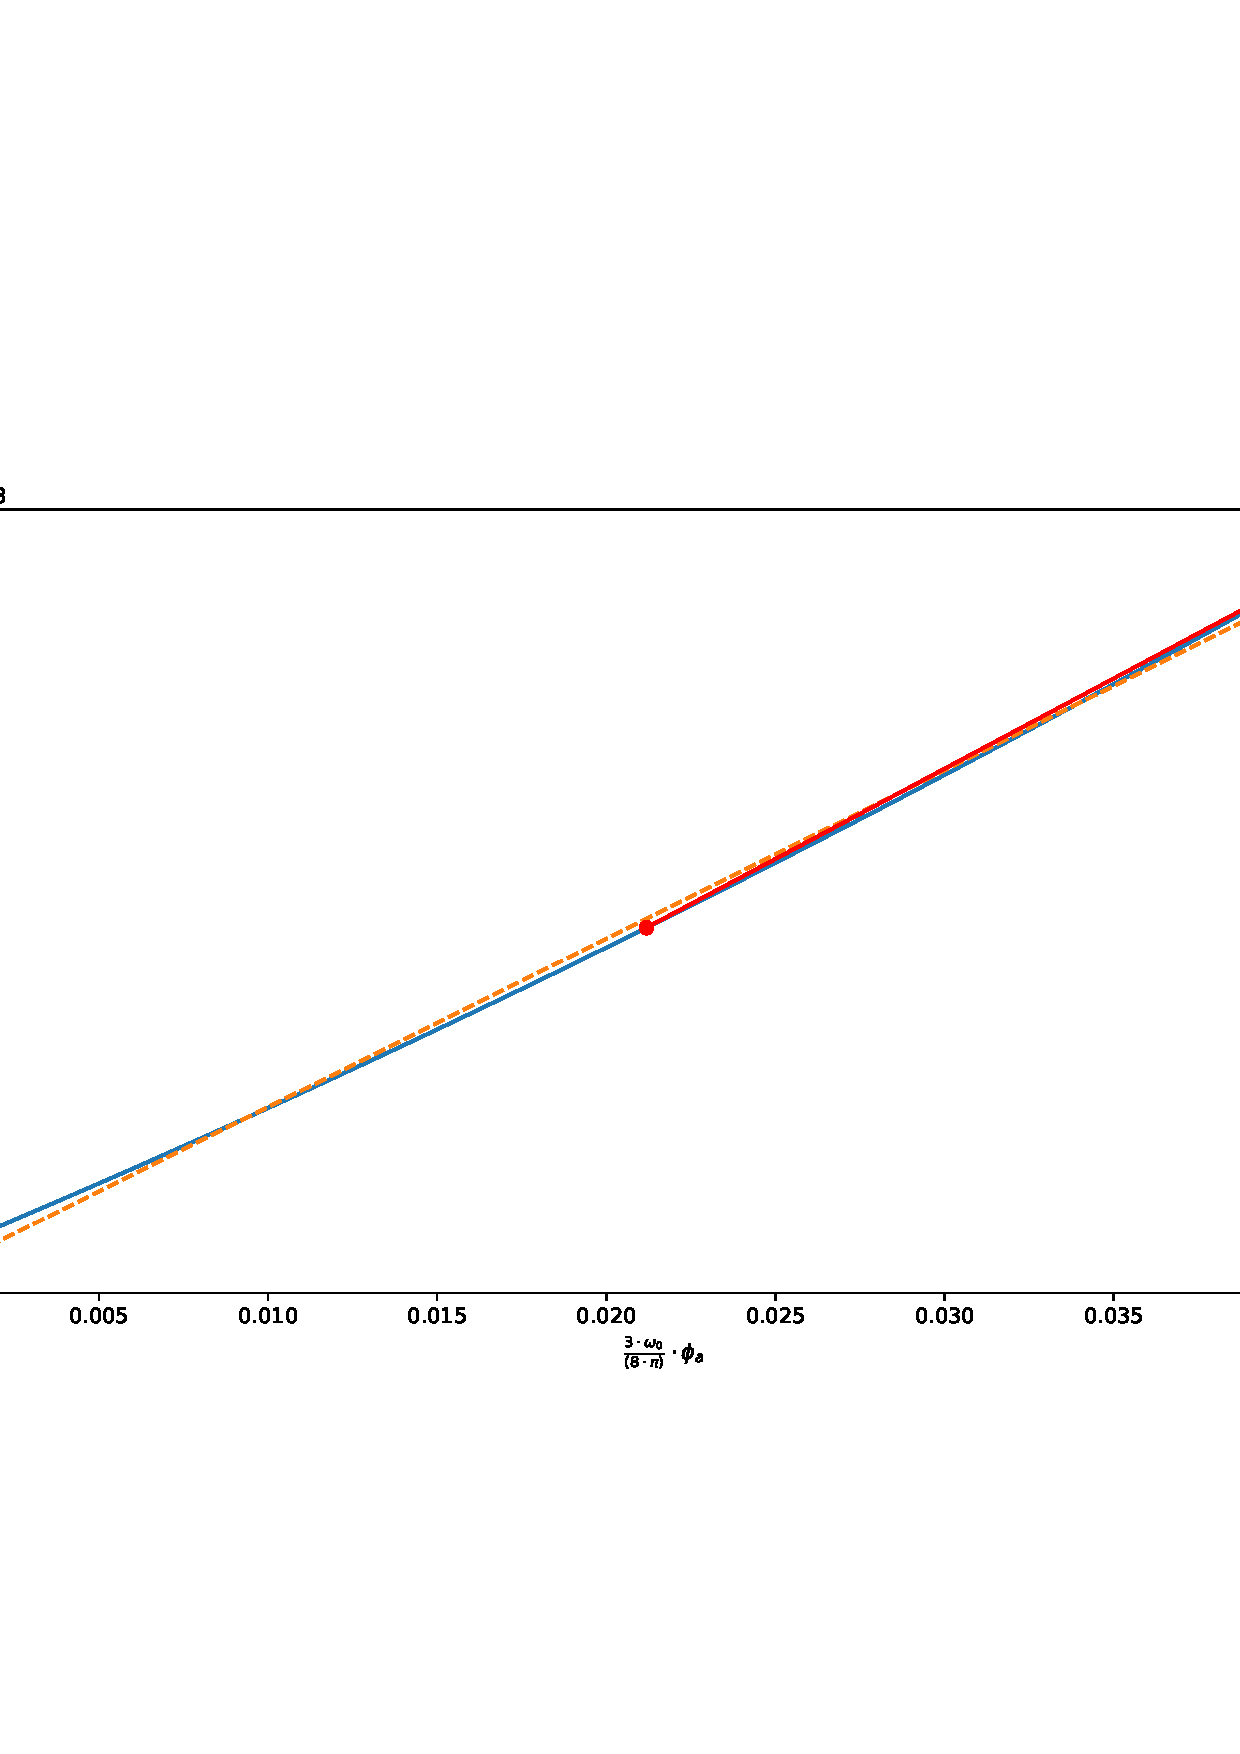
\includegraphics[height=5cm, width=8cm]{figures/ikeda_B_1_B_2.pdf}
    \vspace{-0.5cm}
    \caption{Variation of roll amplitude to derive $B_1$ and $B_2$}
    \label{fig:ikeda_B_1_B2}
\end{figure}

\begin{figure}[H]
    \centering
    \includegraphics[height=13cm, width=15cm]{figures/ikeda_variation.pdf}
    \caption{Simplified method parameter variation}
    \label{fig:ikeda_variation}
\end{figure}







